\documentclass[10pt,a4paper]{article}
\usepackage[utf8]{inputenc}
\usepackage{amsmath}
\usepackage{amsfonts}
\usepackage{amssymb}
\usepackage{graphicx}
\graphicspath{{img//}}
\pagestyle{headings}

\author{Antonia Wagner \and Daniel Buth \and Johannes Müller \\ \\
Fachbereich Angewandte Informatik der Hochschule Fulda\\ \\
Modul \textit{Soft Computing}\\
Prof. Dr. Oleg Taraszow\\ \\
Betreuer: Lukas Militz
}
\title{Fuzzygesteuerte U-Bahn Simulation}
\date{Wintersemester 2010/11}

\makeindex

\begin{document}

\maketitle
\tableofcontents

\section{Projektrahmen}
\subsection{Aufgabenstellung}
\begin{abstract}
Unsere Aufgabenstellung war es, im Rahmen des Praktikums zur Lehrveranstaltung \textit{Soft Computing} bei Prof. Dr. Oleg Taraszow einen Fuzzy-Regler zu erstellen.
Als Werkzeug stand uns dazu die \textit{Fuzzy-Toolbox} der Software \textit{Matlab} zur Verfügung.
Optionale Bonusaufgabe war die Erstellung eines Java-Applets zur Visualisierung.
\end{abstract}

\begin{figure}[htb]
\begin{itemize}
	\item Eingangsvariablen: mindestens 3, mindestens 15 Terme
	\item Ausgangsvariablen: mindestens 2, mindestens 8 Terme
	\item Regeln: mindestens 25
\end{itemize}
\caption{Projektvorgaben}
\label{projektvorgaben}
\end{figure}

\subsection{Projektrahmen}
Bei Bewegungen kommen an vielen Stellen unscharfe Werte vor wie beispielsweise Geschwindigkeit, Entfernungen und Veränderungen dieser Parameter. Daher wollten wir unser Projekt im Bereich Verkehr ansiedeln.
Eine der ersten größere Anwendungen eines Fuzzy-Reglers in der Praxis die automatisierte Anfahr--, Beschleunigungs-- und Bremssteuerung der U-Bahn Sendai in Japan und wir entschieden uns, ein ähnliches Konzept umzusetzen.

\begin{figure}[htb]
\begin{center}
\leavevmode
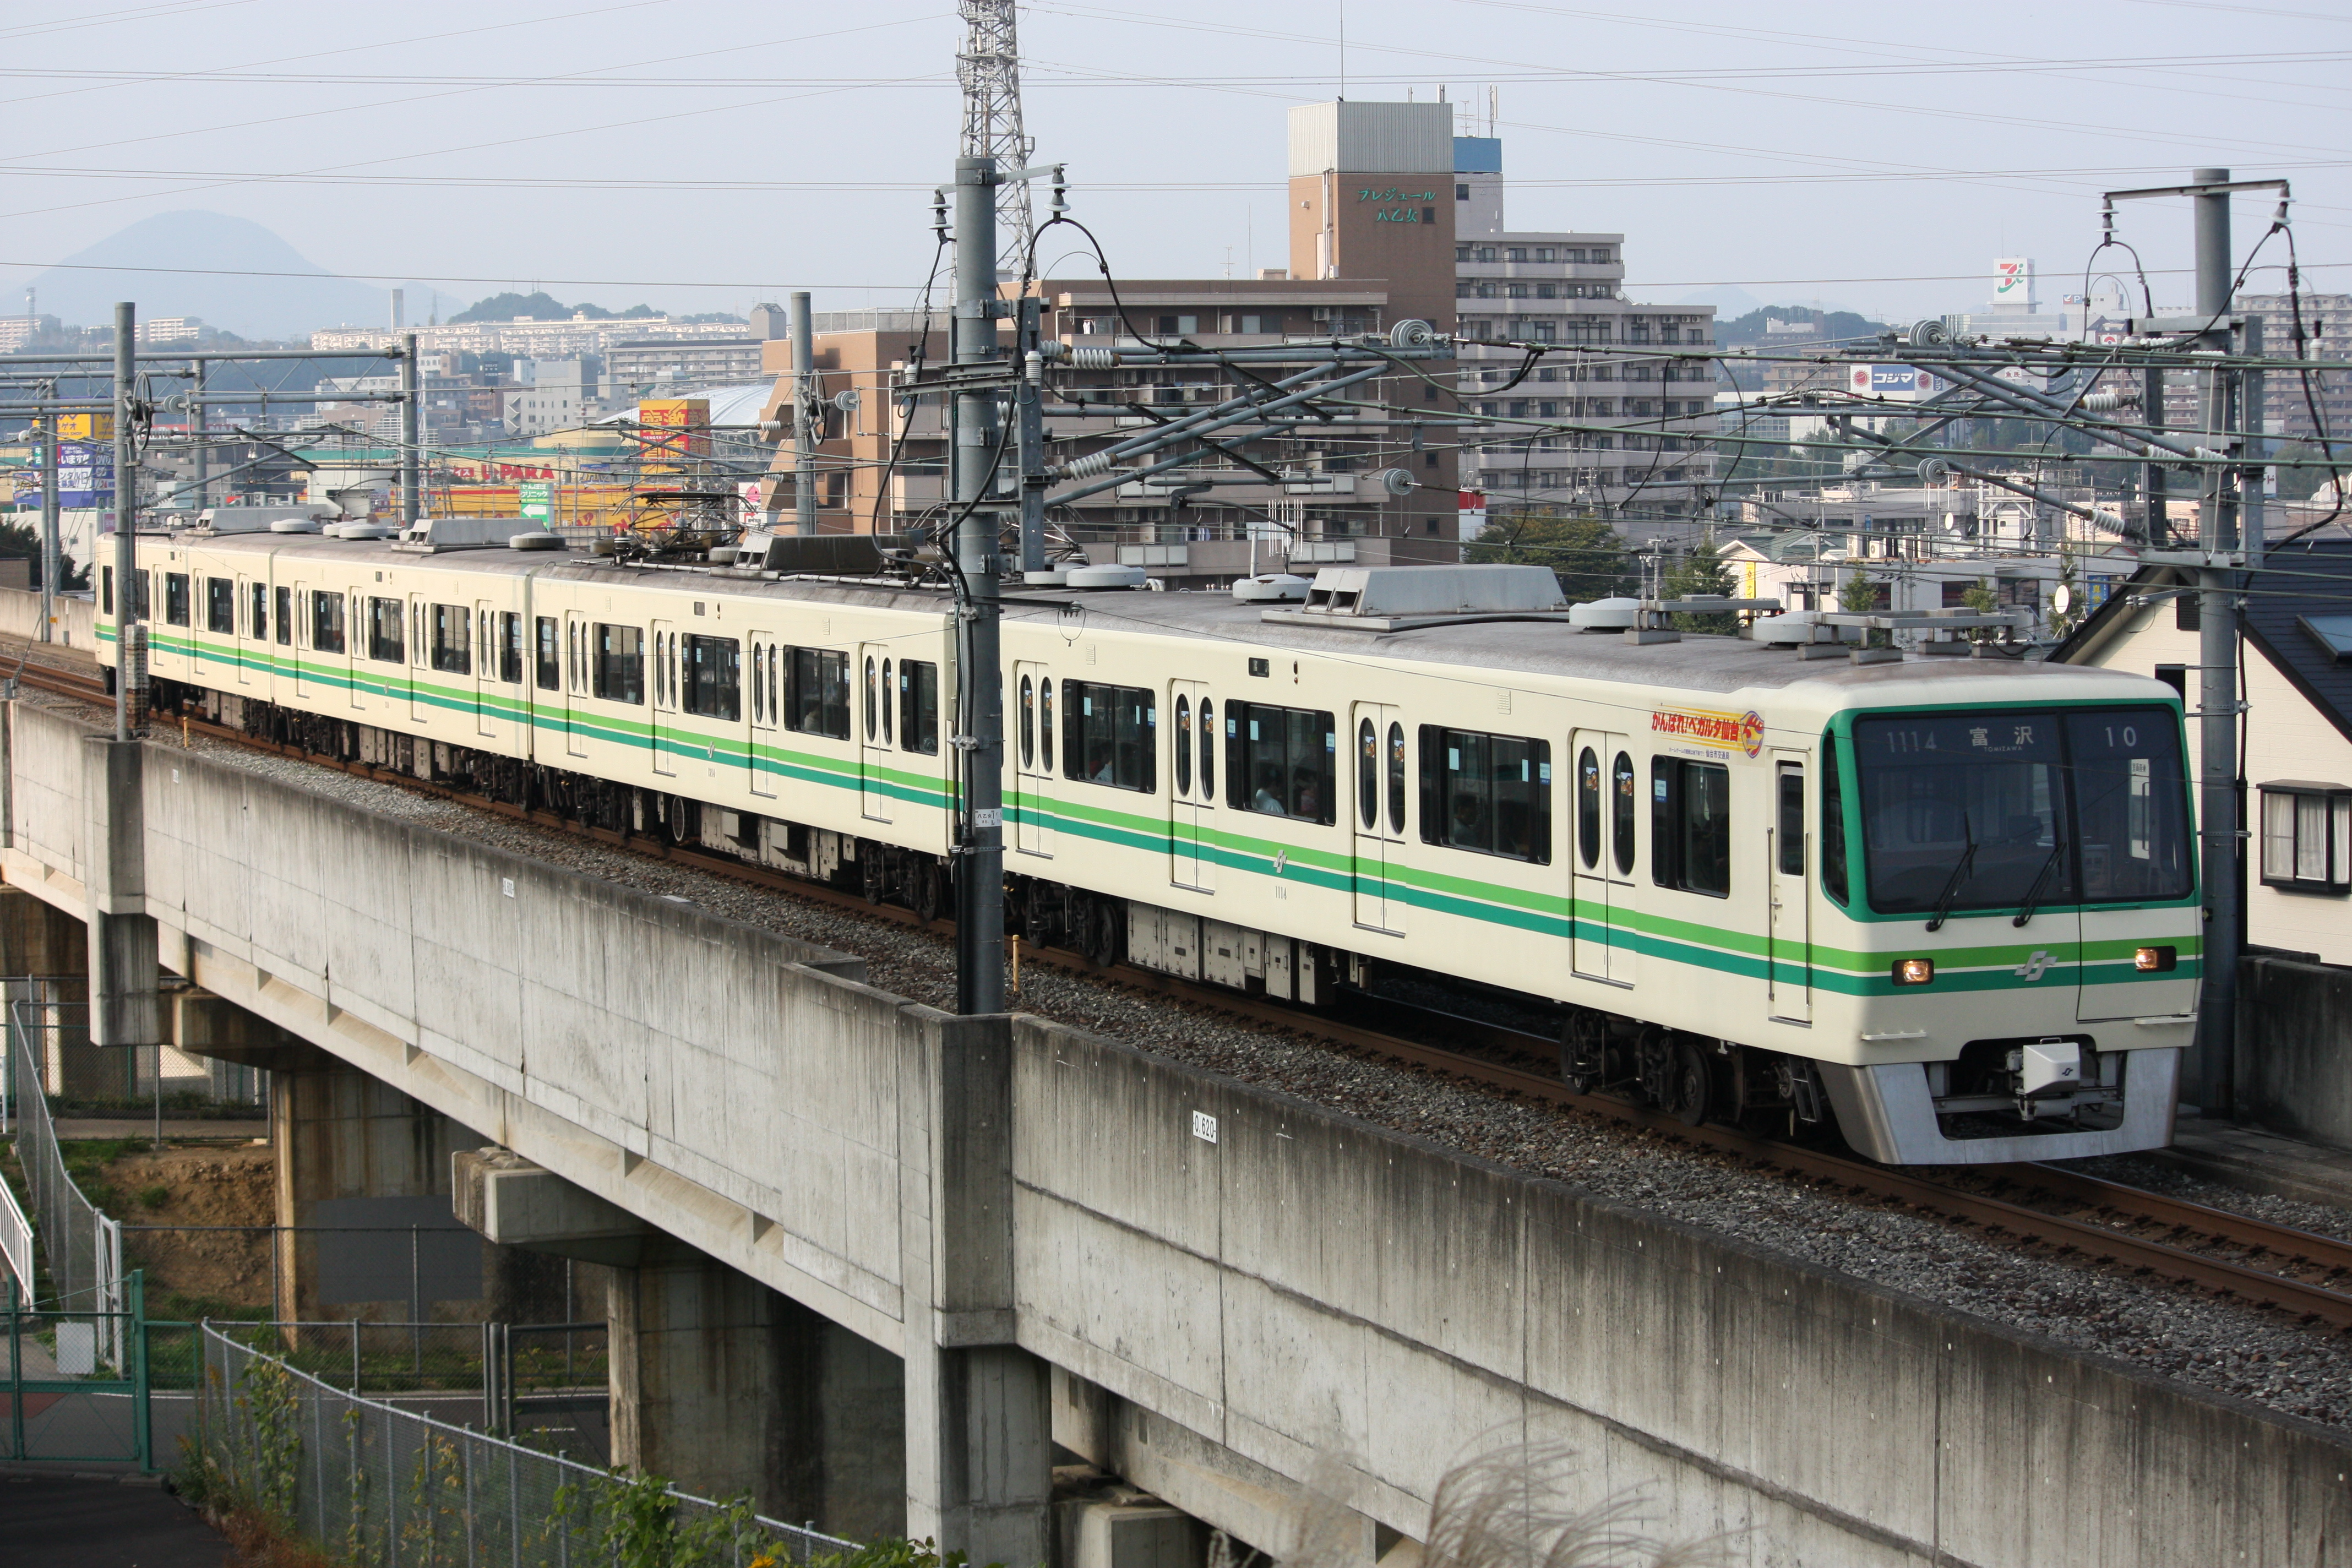
\includegraphics[width=.8\textwidth]{Sendai_subway_1014_20081021.jpg}
\caption[Sendai Subway]{Sendai Subway}
\label{Sendai Subway}
\footnote{Quelle: Wikimedia Commons}
\end{center}
\end{figure}

Unser Projekt sollte die Fahr- und Bremssteuerung eines schienengebundenen Verkehrsmittels wie eine U-Bahn mittels Fuzzy-Logic umsetzen.
Im Gegensatz zum Pionierprojekt der U-Bahn Sendai wollten wir jedoch eine komplette Fahrzeugsteuerung mittels Fuzzy-Regler erreichen.
\paragraph{}
Durch unseren Regler sollte das gesteuerte Fahrzeug in der Lage sein, aus dem Stillstand anzufahren und bis zu einer bestimmten, festgesetzten Geschwindigkeit zu beschleunigen und diese zu halten. Bei auf der Strecke voraus liegenden Wegpunkten wie eine Haltestelle oder ein Signal mit Haltbegriff soll ein Bremsvorgang eingeleitet werden, der das Fahrzeug möglichst sanft und punktgenau zum Stehen bringt.
\paragraph{}
Ebenso sollte es möglich sein, eine beliebige Geschwindigkeit erreichen und halten zu können. Dies kann beispielsweise bei einem langsameren vorausfahrenden Fahrzeug nötig sein. Auch die Einrichtung einer Langsamfahrstrecke kann ein solches Verhalten erfordern.
\paragraph{}
Zusätzlich zur eigentlichen Projektaufgabe haben wir uns zudem als Ziel gesetzt, als Bonusaufgabe eine Anwendung unseres Reglers als Java-Applet zu realisieren.

\section{Vorüberlegungen}
\subsection{Szenario}

Um das Projekt überschaubar zu halten, beschränkten wir unser Szenario auf den ganz einfachen Fall eines linearen, ebenen Streckenverlaufs ohne Abzweigungen oder sonstige andersgeartete Einflüsse. Auf dieser Strecke können sich einzig Hindernisse wie Haltestellen, vorausfahrende Züge oder Geschwindigkeitsbegrenzungen befinden. Das Fahrzeug sollte nur in der Lage sein, vorwärts zu fahren, sowie Beschleunigungs-- und Bremsvorgänge auszuführen. Ein Fahrtrichtungswechsel ist nicht vorgesehen.

\subsection{Fuzzy-Regler}

\subsubsection{Eingangsvariablen}
Als Eingangsvariablen wählten wir zunächst die einfachen Fahrzeugparameter der aktuellen Geschwindigkeit sowie die Entfernung zum nächsten Hindernis. Diese Variablen allein würden schon genügen, um ein einfaches Stop-and-Go-Verhalten zu erreichen, bei dem das Fahrzeug an jedem Punkt auf seinem Weg anhält um dann ggf. wieder neu anzufahren.
\newline
Dies reichte uns allerdings nicht aus, da auch die Geschwindigkeitskomponente des Zielobjektes berücksichtigt werden sollte, wenn es sich um einen vorausfahrendes Fahrzeug handelt oder eine Geschwindigkeitsbegrenzung erreicht werden soll.
Die Verarbeitung der konkreten Geschwindigkeit des Zielobjekts im Regler würde allerdings zu einer unüberschaubaren Fülle an Kombinationen von aktueller und zu erreichender Geschwindigkeit führen. Daher führten wir stattdessen den Geschwindigkeitsunterschied als Differenz von Zielgeschwindigkeit und aktueller Fahrzeuggeschwindigkeit als Variable ein.
\paragraph{Wertebereiche}
Die aktuelle Geschwindigkeit beträgt mindestens $ 0\, km/h $. Als zulässige Streckenhöchstgeschwindigkeit legten wir U-Bahn-typische $ 80\, km/h $ fest, um auch leichte Überläufe erlauben zu können, vergrößerten wir den Wertebereich allerdings noch um ein gutes Stück auf $ 120\, km/h $.

\begin{figure}[htb]
\begin{center}
\includegraphics[width=.5\textwidth]{var_speed.png}
\caption[Eingangsvariable Geschwindigkeit]{Terme der Eingangsvariable Geschwindigkeit}
\label{var_speed}
\end{center}
\end{figure}

Den Wertebereich für die Entfernung des Ziels legten wir fest auf den Bereich von $ 0 - 1500 \, m $ wodurch ein genügend weiter Ausblick auf die vor dem Zug liegende Strecke gewährleistet ist.

\begin{figure}[htb]
\begin{center}
\includegraphics[width=.5\textwidth]{var_target_distance.png}
\caption[Eingangsvariable Zielentfernung]{Terme der Eingangsvariable Zielentfernung}
\label{var_target_distance}
\end{center}
\end{figure}

Analog zur aktuellen Geschwindigkeit liegt die Geschwindigkeitsdifferenz zwischen der Höchstgeschwindigkeit und dem betragsgleichen negativen Wert.

\begin{figure}[htb]
\begin{center}
\includegraphics[width=.5\textwidth]{var_target_speed.png}
\caption[Eingangsvariable Geschwindigkeitsdifferenz]{Terme der Eingangsvariable Geschwindigkeitsdifferenz}
\label{var_target_speed}
\end{center}
\end{figure}

\subsubsection{Ausgangsvariablen}
Auf die Geschwindigkeit beziehungsweise die Beschleunigungsvorgänge eines elektrisch betriebenen Schienenfahrzeugs haben zwei Komponenten wesentlichen Einfluss: Der Fahrmotor sowie die Betriebsbremse (Druckluftbremse).
\paragraph{Zum Beschleunigen} wird die Leistung des Fahrmotors erhöht, wodurch elektrische Energie in Bewegungsenergie umgesetzt wird. Um eine Geschwindigkeit beizubehalten (Nullbeschleunigung) genügt es, den Fahrmotor für eine geringe Leistungsabgabe anzusteuern, da lediglich die durch die Bewegung verlorene Reibungsverluste ausgeglichen werden müssen. Wenn der Motor in den Leerlauf schaltet, sinkt die Geschwindigkeit kontinuierlich ab.

\paragraph{Beim Bremsen} (negative Beschleunigung) wirkt einerseits die Betriebsbremse, die je nach gewünschter Bremsstärke durch druckluftbetriebene Bremszylinder eine Bremskraft auf die Radachsen bewirkt. Im Regelbetrieb wird die zur Verfügung stehende Bremskraft nur zu einem Bruchteil beansprucht, volle Leistung wird nur bei einer Notbremsung abgerufen.
\newline 
\newline
Zudem kommt beim Bremsen eine Besonderheit des Elektromotors zum Tragen: Die elektrische Bremswirkung, die eintritt, wenn ein Elektromotor in den Generatorbetrieb umgeschaltet wird. Dieser Vorteil einer stufenlosen und verschleißarmen Bremswirkung wird in der Praxis bei nahezu allen elektrischen Triebfahrzeugen eingesetzt, erreicht allerdings keine so starke Bremsbeschleunigung wir eine mechanische Bremse, weshalb diese stets zusätzlich vorhanden sein muss und bei stärkeren Bremsvorgängen additiv zugeschaltet wird.
Auf in der Praxis oftmals zusätzlich verwendete weitere Bremssysteme wurde im Zuge der Vereinfachung verzichtet.

\paragraph{Wertebereiche}
Als Wertebereiche verwendeten wir für die Motorsteuerung den Bereich $ -100 \% $ und $ +100 \% $ während die Bremsstärke zwischen $ 0 \% $ und $ 100 \% $ liegt.

\paragraph{}
Damit waren die Projektvorgaben (siehe \ref{projektvorgaben}) erfüllt.

\section{Umsetzung}

\subsection{Fuzzy-Toolbox}

\subsection{Applet}

\subsubsection{Dynamikberechnungen}
\begin{equation}
E_{kin} = \frac{1}{2} m v^{2} 
\end{equation}

\begin{equation}
\bigtriangleup E = \bigtriangleup t \ast \bigtriangleup E
\end{equation}

\paragraph{Betrachtung bezogen auf die Zeit}
\begin{equation}
E_{kin}(t_{1}) = E_{kin}(t_{2}) + \bigtriangleup t \ast P_{eff}
\end{equation}

\begin{equation}
v_{1} = \sqrt{v_{0}^2 + 2 \bigtriangleup t \frac{P_{eff}}{m}}
\end{equation}

\paragraph{Fahrwiderstände}

Zur Berechnung der Fahrwiderstände wurden jeweils die entsprechenden Grundformeln, aber stark vereinfacht eingesetzt.

\begin{equation}
W_F = W_R + W_L
\end{equation}
Der Fahrwiderstand des Zuges besteht aus dem Rollwiderstand auf ebener und gerader Fahrbahn und dem Luftwiderstand.
\subparagraph{Rollwiderstand}
\begin{equation}
W_R = c_w \ast m * g \\
\end{equation}
mit $ c_w \approx 0.0015 $
\subparagraph{Luftwiderstand}
\begin{equation}
W_L = \frac{p_{Luft}}{2} * c_w * A * v^2
\end{equation}
mit $ A \approx 10 m^2 $ und $ p_{Luft} \approx 1.2 $

\subparagraph{Streckenwiderstände} konnten komplett außer acht gelassen werden, da unser Szenario nur eine gerade, ebene, linear trassierte Strecke vorsieht, und daher keine Steigungs--, Neigungs-- oder Krümmungswiderstände auftreten.

\subparagraph{Beschleunigungswiderstand}
\begin{equation}
W_B = m * a
\end{equation}

\paragraph{Traktionsleistung}
\begin{equation}
P_{eff} = \sum W * v
\end{equation}

\subsubsection{Fahrzeugparameter}
Um die Berechnungen mit realistischen Werten durchführen zu können, erhielt unser Testfahrzeug typische Fahreigenschaften eines U-Bahn-Fahrzeugs. Insbesondere lehnten wir uns an die \textit{Baureihe B} der U-Bahn München und die \textit{Baureihe H} der U-Bahn Berlin an.

\begin{figure}
\begin{center}
\begin{tabular}{|lr|}
\hline \textbf{Eigenschaft} & \textbf{Wert} \\ 
\hline Masse & $ 80\, t$ \\ 
\hline Länge & $ 40\, m$ \\ 
\hline Höchstgeschwindigkeit & $ 80 \, km/h $ \\ 
\hline Nennleistung & $ 780 \, kW $ \\ 
\hline maximale Bremskraft & $ 100 \, kN $ \\ 
\hline 
\end{tabular} 
\end{center}
\caption{Datenblatt unserer Testfahrzeugs}
\label{datenblatt}
\end{figure}

\section{Zusammenfassung}

\end{document}